% Standalone TikZ figure: Prefill (GEMM) vs Decode (GEMV)
% Shows that prefill processes all tokens at once (matrix) while decode processes one token at a time (vector)
\documentclass[tikz,border=2pt]{standalone}
\usepackage{tikz}
\usetikzlibrary{positioning,arrows.meta,decorations.pathreplacing}
\usepackage{amsmath}

\begin{document}
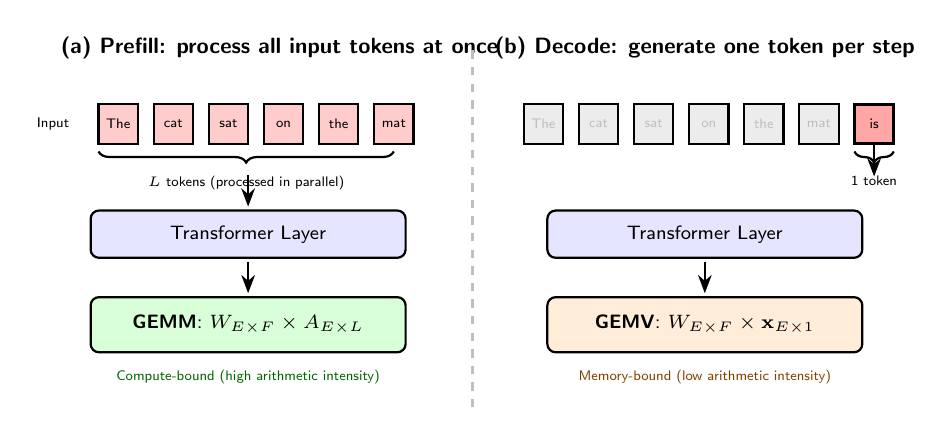
\begin{tikzpicture}[
    >=Stealth,
    font=\sffamily\scriptsize,
    token/.style={draw, thick, minimum width=0.5cm, minimum height=0.5cm, inner sep=0pt},
    phase/.style={font=\sffamily\footnotesize\bfseries},
  ]

  % ============================================================
  % (a) Prefill Phase — all tokens processed at once → GEMM
  % ============================================================
  \node[phase, anchor=south] at (2.4, 4.2) {(a) Prefill: process all input tokens at once};

  % Input prompt tokens
  \node[font=\sffamily\tiny, anchor=east] at (-0.15, 3.5) {Input};
  \foreach \i/\t in {0/The, 1/cat, 2/sat, 3/on, 4/the, 5/mat} {
    \node[token, fill=red!20] (pt\i) at (\i*0.7+0.35, 3.5) {\tiny \t};
  }

  % Brace under tokens
  \draw[decorate, decoration={brace, mirror, amplitude=4pt}, thick]
    (0.1, 3.15) -- (3.85, 3.15)
    node[midway, below=5pt, font=\sffamily\tiny] {$L$ tokens (processed in parallel)};

  % Arrow down to transformer
  \draw[->, thick] (2.0, 2.85) -- (2.0, 2.45);

  % Transformer block
  \node[draw, thick, fill=blue!10, rounded corners=3pt,
        minimum width=4.0cm, minimum height=0.6cm] (tf1) at (2.0, 2.1)
    {Transformer Layer};

  % Arrow down to GEMM
  \draw[->, thick] (2.0, 1.75) -- (2.0, 1.35);

  % GEMM operation box
  \node[draw, thick, fill=green!15, rounded corners=3pt,
        minimum width=4.0cm, minimum height=0.7cm] (gemm) at (2.0, 0.95)
    {\textbf{GEMM}: $W_{E \times F} \times A_{E \times L}$};

  % Label
  \node[font=\sffamily\tiny, text=green!40!black, anchor=north] at (2.0, 0.5)
    {Compute-bound (high arithmetic intensity)};

  % ============================================================
  % (b) Decode Phase — one token at a time → GEMV
  % ============================================================
  \node[phase, anchor=south] at (7.8, 4.2) {(b) Decode: generate one token per step};

  % Already generated tokens (grayed out)
  \foreach \i/\t in {0/The, 1/cat, 2/sat, 3/on, 4/the, 5/mat} {
    \node[token, fill=gray!15, text=gray!50] (dt\i) at (\i*0.7+5.75, 3.5) {\tiny \t};
  }
  % Current single token being processed (highlighted)
  \node[token, fill=red!35, line width=1pt] (dcur) at (6*0.7+5.75, 3.5) {\tiny is};

  % Brace under single token
  \draw[decorate, decoration={brace, mirror, amplitude=4pt}, thick]
    (9.7, 3.15) -- (10.2, 3.15)
    node[midway, below=5pt, font=\sffamily\tiny] {1 token};

  % Arrow down to transformer
  \draw[->, thick] (dcur.south) -- ++(0, -0.4);

  % Transformer block
  \node[draw, thick, fill=blue!10, rounded corners=3pt,
        minimum width=4.0cm, minimum height=0.6cm] (tf2) at (7.8, 2.1)
    {Transformer Layer};

  % Arrow down to GEMV
  \draw[->, thick] (7.8, 1.75) -- (7.8, 1.35);

  % GEMV operation box
  \node[draw, thick, fill=orange!15, rounded corners=3pt,
        minimum width=4.0cm, minimum height=0.7cm] (gemv) at (7.8, 0.95)
    {\textbf{GEMV}: $W_{E \times F} \times \mathbf{x}_{E \times 1}$};

  % Label
  \node[font=\sffamily\tiny, text=orange!50!black, anchor=north] at (7.8, 0.5)
    {Memory-bound (low arithmetic intensity)};

  % ============================================================
  % Divider
  % ============================================================
  \draw[dashed, gray!50, thick] (4.85, -0.1) -- (4.85, 4.5);

\end{tikzpicture}
\end{document}
